%% LyX 1.3 created this file.  For more info, see http://www.lyx.org/.
%% Do not edit unless you really know what you are doing.
\documentclass[12pt,english]{article}
\usepackage[T1]{fontenc}
\usepackage[latin1]{inputenc}
\usepackage{graphicx}
\usepackage{amssymb}

\makeatletter

%%%%%%%%%%%%%%%%%%%%%%%%%%%%%% LyX specific LaTeX commands.
%% Bold symbol macro for standard LaTeX users
\providecommand{\boldsymbol}[1]{\mbox{\boldmath $#1$}}


%%%%%%%%%%%%%%%%%%%%%%%%%%%%%% User specified LaTeX commands.
\usepackage{amssymb,epsfig,capt-of,ifthen,calc}

%%%%%%%%%% Start TeXmacs macros
\newcommand{\tmfloatcontents}{}
\newlength{\tmfloatwidth}
\newcommand{\tmfloat}[5]{
  \renewcommand{\tmfloatcontents}{#4}
  \setlength{\tmfloatwidth}{\widthof{\tmfloatcontents}+1in}
  \ifthenelse{\equal{#2}{small}}
    {\ifthenelse{\lengthtest{\tmfloatwidth > \linewidth}}
      {\setlength{\tmfloatwidth}{\linewidth}}{}}
    {\setlength{\tmfloatwidth}{\linewidth}}  \begin{minipage}[#1]{\tmfloatwidth}
    \begin{center}
      \tmfloatcontents
      \captionof{#3}{#5}
    \end{center}
  \end{minipage}}
%%%%%%%%%% End TeXmacs macros


\usepackage{babel}
\makeatother
\begin{document}

\title{Insurance}


\author{Michael Peters}


\date{\today{}}

\maketitle

\section{Introduction}

In this chapter, we study a very simple model of insurance using the
ideas and concepts developed in the chapter on risk aversion. You
may recall from the previous chapter, the concept of a \emph{lottery}:
a collection of outcomes that are each assigned a different probability
of occurring. We are going to assume that the independence axiom holds,
and that our consumers and decision makers have preferences that are
linear in the probabilities with which these different outcomes occur.

Expected utility says that we should start with a list of all possible
\emph{outcomes}. Let's just think of the set of outcomes as a finite
set $S$ (later on we will refer to them as \emph{states}). Sometimes,
we let $S$ refer to the number of outcomes in this set. We let $s$
refer to a particular outcome in this set. A lottery is a vector of
probabilities $p$ consisting of $S$ non-negative components, the
sum of which must equal $1.$ The expected utility theorem says that
there is a vector of real numbers $\{ u_{1},\ldots,u_{S}\}$ such
that two lotteries $p$ and $q$ can be ranked in the following way:
$p\succeq q$ if and only if \[
\sum_{s=1}^{S}p_{s}u_{s}\geqslant\sum_{s=1}^{S}q_{s}u_{s}\]
 In most of what we do in economics, including the insurance problem,
we fix the probabilities $p$ then vary the numbers $u_{s}$ in some
fashion. This is exactly what we are going to do here with the insurance
problem.

On the surface, the expected utility theorem doesn't seem to support
this approach. In fact, it is a very restrictive special case which
you can understand if you think of the set of outcomes as a continuum,
and the set of lotteries as a set of probability measures on this
continuum. At the moment, the details of this argument aren't so important.
All you need to remember is that we will use the expected utility
theorem to support the arguments here.

Let's apply these ideas to insurance. We start with a consumer who
has an income $y$ but who expects to have an accident with some probability
$p$. The accident has a known monetary cost $d$. The consumer deals
with a competitive insurance company which sells policies to many
similar consumers and knows the probability with which the consumer
has an accident.

A good example might be a farmer whose fields produce a yearly income
$y$ unless there is a late frost which kills off some of his crop.
The probability of a late frost is $p$. A bad example would be car
insurance. There are a couple of reasons why. The first is that the
probability of an accident is something that a driver has some control
over. If you are insured against the costs of an accident, then there
is little incentive to take care. This is referred to as \emph{moral
hazard}. A farmer, on the other hand, has little control over the
weather. Drivers also have a lot of information about their own accident
probability that the insurance company doesn't. The weather, on the
other hand, is unpredictable, but in a way that everyone agrees.

The insurance company will sell a \emph{policy} to the consumer. A
policy is a premium $q$ and a \emph{net} benefit $b$. The net benefit
is the difference between the gross benefit $B$ and the premium $q.$
The way the insurance policy works is that the consumer pays the insurance
company $q$ up front. Then, if (and only if) the consumer has an
accident, the insurance company pays the consumer $B$. Equivalently,
if the consumer has an accident, the insurance company pays back the
premium $q$ and gives the consumer an additional $b$ to make up
for her loss.

The insurance company is doing this with many different consumers
and is willing to offer the consumer any policy that breaks even in
the sense that the company's expected profit from the policy is zero.
The expected profit to the company from a policy with premium $q$
and net benefit $b$ is \[
(1-p)q-pb\]


Our consumer has expected utility preferences, so if she buys a policy
with premium $q$ and net benefit $b$, her expected utility is \[
(1-p)u(y-q)+pu(y-d+b)\]
 The consumer's problem is to buy a policy that maximizes her expected
utility.

Let's solve the problem two different ways. First, we use the graphical
approach. To see this approach, we can convert the problem into something
that looks exactly like the consumer problems we have already studied.

%
\begin{figure}
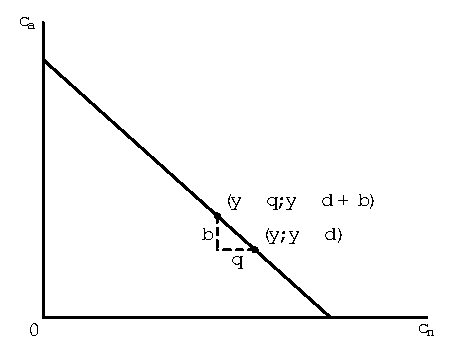
\includegraphics{insurance_fig1.eps}


\caption{Budget Set\label{fig1}}
\end{figure}


The horizontal axis in the diagram measures the amount of income the
consumer enjoys in the event that she does not have an accident. If
she doesn't buy insurance, this will just be $y$. If she does buy
insurance, it will be $y$ less the premium that she pays. The vertical
axis measures the level of consumption in the event that our consumer
does have an accident. In this diagram, the consumer's \emph{endowment}
is the point $(y,y-d)$. The consumer can switch from her endowment
to the consumption pair $(y-q,y-d+b)$ by buying a policy with premium
$q$ and net benefit $b$.

In the diagram, I have drawn this as if it created an entire budget
line for the consumer. The reasoning is as follows: the insurance
company will presumably be willing to sell the consumer \emph{any}
policy that generates zero expected profit, i.e., any policy that
satisfies $(1-p)q-pb=0$, or $b=q\frac{1-p}{p}$. The set of all such
policies generates a feasible set that passes through the endowment
point (since the policy $(0,0)$ obviously gives the insurance company
zero expected profit) and has slope $-\frac{1-p}{p}$.

The consumer's indifference curves are made up of all the pairs $(c_{n},c_{a})$
that yield the same level of expected utility. So for example, the
indifference curve through the endowment is given by the set of solutions
to \begin{equation}
(1-p)u(c_{n})+pu(c_{a})=(1-p)u(y)+pu(y-d)\end{equation}
 Using the method of total differentials, the slope of the indifference
curve can be derived by solving \begin{equation}
(1-p)u'(c_{n})dc_{n}+pu'(c_{a})dc_{a}=0\end{equation}
 or \begin{equation}
\frac{dc_{a}}{dc_{n}}=-\frac{(1-p)u'(c_{n})}{pu'(c_{a})}\end{equation}
 A very nice property of expected utility preferences is that if $c_{a}=c_{n}$,
then $u'(c_{a})=u'(c_{n})$. If, in addition, the function $u$ is
concave (has a decreasing first derivative), then the indifference
curves will appear as convex curves as in the following picture:

%
\begin{figure}
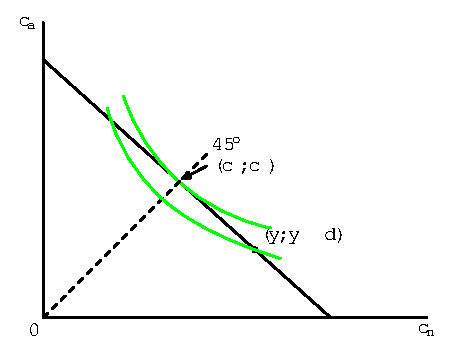
\includegraphics{insurance_fig2.eps}


\caption{Constant Consumption\label{fig2}}
\end{figure}


Since the slope of every indifference curve is $-\frac{1-p}{p}$ on
the $45^{o}$ line, the highest indifference curve's tangency point
to the budget set will occur on the $45^{o}$ line. The nice implication
is that a risk averse consumer who can buy insurance at `actuarially
fair' prices (i.e., prices that give the insurance company zero expected
profit) will buy insurance up to the point where his consumption is
the same whether or not she has an accident.

To be complete, let's solve this as well using Lagrangian methods
because it proves insightful. First, the consumers problem (at least
when dealing with a fair insurance company) is to maximize \begin{equation}
(1-p)u(y-q)+pu(y-d+b)\end{equation}
 by choosing a premium and benefit package $(q,b)$ subject to the
constraint that \begin{equation}
(1-p)q-pb=0\end{equation}
 Notice that there is nothing here about the premium and benefit being
positive. It is conceivable that the consumer might want to bet with
another consumer that she would \emph{not} have an accident. In that
case, she would receive money from the other consumer when she didn't
have an accident, which coincides with a negative value for $q$.
Then, to satisfy the constraint, she would have to pay out in the
event that she did have an accident.

Since there are no inequality constraints, our Lagrangian theorem
says that at the optimal solution, there will be a multiplier $\lambda$
such that \begin{equation}
-(1-p)u'(y-q)+\lambda(1-p)=0\end{equation}
 and \begin{equation}
pu'(y-d+b)-\lambda p=0\end{equation}
 The probabilities cancel in this expression, so we get $u'(y-q)=u'(y-d+b)=\lambda$.
If we assume that the marginal utility of income is monotonically
declining, then this can only occur when $y-q=y-d+b$.
\end{document}
